\documentclass[11pt,a4paper]{article}

\usepackage{iftex}
\ifPDFTeX
  \usepackage[utf8]{inputenc}
  \usepackage[T1]{fontenc}
  \usepackage[scaled=0.95]{helvet}
  \usepackage{microtype}
\else
  \usepackage{fontspec}
  \setmainfont{Arial}
  \setsansfont{Arial}
\fi

\usepackage[brazil]{babel}
\usepackage[a4paper,top=2.5cm,bottom=2.5cm,left=3.0cm,right=3.0cm]{geometry}
\usepackage{graphicx}
\usepackage{float}
\usepackage{array}
\usepackage{tabularx}
\usepackage{xcolor}
\usepackage{enumitem}
\usepackage{setspace}
\usepackage[hidelinks]{hyperref}

\renewcommand{\familydefault}{\sfdefault}

% Cor exata dos títulos observada no relatorio.pdf original (#0F4761 / RGB 0.0588, 0.278, 0.38)
\definecolor{headingBlue}{HTML}{0F4761}
\definecolor{tableGrid}{HTML}{888888}

% Documento limpo sem cabeçalho, rodapé ou numeração de páginas, idêntico ao relatorio.pdf
\pagestyle{empty}

\setlength{\parskip}{0pt}
\setlength{\parindent}{1.25cm}
\setstretch{1.42}

\newcommand{\tituloSecao}[1]{%
  \par\addvspace{12pt}%
  {\noindent\fontsize{20pt}{24pt}\selectfont\normalfont\color{headingBlue}#1\par}%
  \vspace{4pt}%
}

\newcommand{\subtituloSecao}[1]{%
  \par\addvspace{10pt}%
  {\noindent\fontsize{16pt}{20pt}\selectfont\normalfont\color{headingBlue}#1\par}%
  \vspace{3pt}%
}

\newcommand{\subsubtituloSecao}[1]{%
  \par\addvspace{8pt}%
  {\noindent\fontsize{13pt}{16pt}\selectfont\bfseries\color{headingBlue}#1\par}%
  \vspace{2pt}%
}

\newcolumntype{L}[1]{>{\raggedright\arraybackslash}p{#1}}
\newcolumntype{C}[1]{>{\centering\arraybackslash}p{#1}}
\newcolumntype{Y}{>{\raggedright\arraybackslash}X}

\begin{document}
\sloppy

% ==============================================================================
% PARTE 1 — REPRODUÇÃO INTEGRAL E IDÊNTICA DO RELATÓRIO ORIGINAL (PÁGINAS 1 A 8)
% ==============================================================================

\tituloSecao{Design Thinking}

\noindent Antes de explicar a solução em si, sua plataforma e tecnologias, vale dar atenção especial ao motivo deste projeto. A ideia de criar um aplicativo voltado para cuidadoras e familiares de pessoas com Alzheimer, com o objetivo de facilitar o acesso à informação e oferecer apoio emocional surgiu por meio de um processo de Design Thinking ilustrado na imagem a seguir:

\begin{figure}[H]
  \centering
  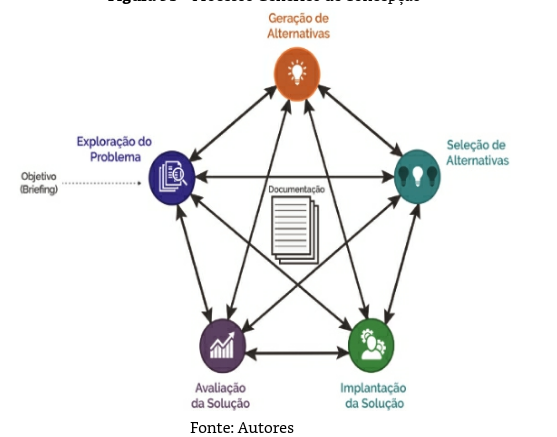
\includegraphics[width=0.50\textwidth]{figuras/img1-design-thinking.png}
\end{figure}

\noindent Ela ressalta o processo não-linear e iterativo do design, possuindo 5 pilares. O grande poder dessa abordagem está em colocar as pessoas reais no centro de tudo: em vez de criar uma solução baseada em achismos, mergulhamos na rotina do usuário para construir algo que realmente resolva a sua dor.

Apesar do processo ter sido executado de maneira não-linear, ou seja, houve um trânsito entre os diversos pilares em momentos distintos, essa parte inicial da documentação terá como objetivo detalhar cada um desses pilares e o que foi feito, ao todo, em cada um deles no intuito de evidenciar a importância e impacto dessa solução proposta, mostrando que há um público-alvo querente dela.

\noindent\textbf{OBS.:} No repositório do GITHUB estarão presentes todos os documentos desenvolvidos ao longo do processo.

\tituloSecao{Exploração do Problema}

\noindent Essa fase consiste essencialmente na compreensão e visão macro do problema, com o intuito de entender a fundo as dores dos stakeholders visando criar uma solução especializada e desejada. Para isso, buscou-se informações em diversas fontes e estilos, como se segue.

\subtituloSecao{Revisão da Literatura (Desk Research)}

\noindent Para fundamentar a exploração do problema de forma científica, conduzi um \textit{Desk Research} composto pelo mapeamento e fichamento de \textbf{12 trabalhos acadêmicos} localizados majoritariamente nos Periódicos da CAPES e na base SciELO, em um processo não linear dividido em duas etapas. A primeira rodada analisou 10 estudos focados nas repercussões biopsicossociais e na sobrecarga global do cuidado, enquanto os 2 últimos artigos refinaram a investigação especificamente sobre alfabetização em saúde, busca ativa por informações e acesso a redes de apoio.

De antemão, vale ressaltar a dificuldade em encontrar dados nacionais sobre o tema. A própria literatura brasileira corrobora essa afirmação, apontando a escassez de estudos nacionais confiáveis sobre o assunto — o que contrasta com países mais desenvolvidos, onde a questão é amplamente estudada. Por esse motivo, a maioria dos artigos brasileiros analisados acaba recorrendo a levantamentos internacionais para embasar seus argumentos. Dados globais da fundação \textit{Alzheimer's Disease International (ADI)} apontam o crescimento contínuo da população idosa, associado ao aumento da expectativa de vida à medida que ocorrem os avanços tecnológicos. Esse crescimento implica diretamente em uma maior quantidade de idosos com doenças neurodegenerativas: cerca de \textbf{47 milhões} de pessoas viviam com algum grau de demência no mundo, sendo \textbf{35,6 milhões} especificamente com a Doença de Alzheimer (DA). Considerando que o \textbf{Brasil é o 6º país com mais idosos no mundo}, percebe-se que a temática é extremamente relevante para o cenário nacional atual (e futuro).

Diante dessa grande quantidade de pessoas com DA, percebe-se que o impacto da condição ultrapassa o próprio enfermo, afetando diretamente seus cuidadores e em especial, os cuidadores informais, compostos por familiares e amigos próximos. A literatura enfatiza que cerca de \textbf{80\%} dos cuidadores de pessoas com Alzheimer são justamente \textbf{informais} e majoritariamente do \textbf{sexo feminino}, evidenciando um forte paralelo com os papéis históricos de gênero. Grande parte dessas cuidadoras sofre com uma sobrecarga intensa, sintetizada em um dos estudos pelo relato chocante: \textit{"Para viver para eles, nós temos que matar a nossa vida"}. Devido às exigências do cuidado, estima-se uma dedicação média de \textbf{60 horas semanais} exclusivas a esse processo, afetando áreas vitais como casamento, profissão, lazer e vida social. Na prática, o familiar passa a acumular tarefas que vão desde a administração financeira e de medicamentos até atividades básicas de higiene pessoal, como dar banho no idoso.

Ademais, os relatos analisados destacam a dificuldade de acesso a bons profissionais da área da saúde que saibam orientar o manejo diário, o alto custo dos medicamentos, a falta de apoio de outros familiares e amigos e a escassez de tempo. Soma-se a isso o despreparo diante da doença, ou seja, a falta de informação acessível e a surpresa repentina que o diagnóstico provoca, transformando a rotina do cuidador de forma abrupta. Destarte, destaca-se a urgência de olhar para a Doença de Alzheimer não somente como uma condição que atinge o paciente, mas essencialmente como algo que adoece quem cuida dele diariamente, visto que a maioria desses cuidadores desenvolve quadros severos de depressão, ansiedade, estresse extremo e fadiga crônica.

\noindent\textbf{Resumo em tópicos:}

\begin{itemize}[leftmargin=1.8cm, itemindent=0pt, label=\textbullet, topsep=4pt, itemsep=2pt]
  \item Aumento da população idosa no mundo, e consequentemente, de DA;
  \item Impacto da doença nos cuidadores, essencialmente nos informais, que compõe a maioria destes;
  \item A maioria dos cuidadores informais são do sexo feminino;
  \item Sobrecarga intensa nos cuidadores informais, cerca de 60 horas semanais dedicados ao processo de cuidado;
  \item Dificuldades dos cuidadores informais: falta de informação, falta de apoio, sobrecarga financeira, sobrecarga temporal etc.;
\end{itemize}

\subtituloSecao{Entrevistas e Imersão em Campo (ABRAz-PE)}

\noindent Para validar se os dados dos artigos refletiam a realidade prática da nossa região, realizei entrevistas divididas em duas rodadas. Na primeira, conversei com 3 cuidadoras informais (Angelúcia, 64 anos; Janey, 59 anos; e Rosanne, 65 anos) que cuidam ou cuidaram de suas mães com Alzheimer. Os relatos bateram exatamente com a literatura: são do sexo feminino, duas delas tiveram que largar a profissão ou se aposentar mais cedo por conta do cuidado, quase não recebiam apoio de outros familiares e sentiam uma exaustão constante. Frases marcantes como \textit{"Tinha dias que não conseguia respirar. Eu quase nunca dormia. Tinha que ficar alerta 24 horas"} e \textit{"Você tem 2 opções com essa doença: deixa morrer ou cuida. Se decidir cuidar, precisa de muito dinheiro"} deixaram claro o peso emocional e financeiro dessa rotina.

Além disso, todas relataram que, ao receberem o diagnóstico, não sabiam quase nada sobre como lidar com a doença no dia a dia, especialmente em momentos críticos como a recusa alimentar, a administração de remédios e a chamada Síndrome do Pôr-do-Sol (confusão e agitação no fim da tarde).

Na segunda rodada, para entender melhor o papel das redes de apoio, entrevistei uma das organizadoras da instituição e também a cuidadora Rosemary (54 anos), participante da ABRAz Pernambuco (Associação Brasileira de Alzheimer).

Destarte, para realizar a fase de \textbf{recrutamento}, fui presencialmente a um evento da ABRAz na Federação Espírita Pernambucana, durante a palestra \textit{"O Comportamento e as Demências"}, ministrada pelo gerontólogo e vice-presidente da ABRAz-PE, Antônio Rodrigues Junior. Isso foi um divisor de águas porque permitiu recrutar 20 cuidadores reais para futuros testes da ferramenta e entrevistas, além da obtenção de dicas práticas valiosas de manejo passadas pelo palestrante, como evitar frases no imperativo.

\begin{figure}[H]
  \centering
  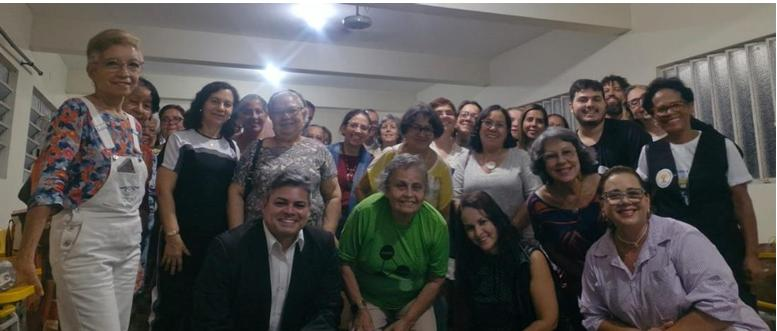
\includegraphics[width=0.92\textwidth]{figuras/img2-imersao-abraz.jpg}
\end{figure}

\subtituloSecao{Mapeamento de Stakeholders, Personas e Jornada do Usuário}

\noindent Com os dados da literatura e das entrevistas em mãos, mapeei os stakeholders envolvidos (cuidadores informais, cuidadores formais, pacientes com DA, governo e acadêmicos), definindo as \textbf{cuidadoras informais} como o público-alvo central da solução.

Para tangibilizar esse público, criei duas personas baseadas diretamente nas histórias reais coletadas. A primeira, \textbf{Maria Falcone (62 anos)}, representa a visão geral da filha que se aposentou para cuidar da mãe, sofre com o afastamento dos amigos e sente falta de aplicativos voltados para o tema (\textit{"Avançaram tanto em aplicativos como Tinder, mas cadê os de Alzheimer?"}). A segunda, \textbf{Valdenice Silva (52 anos)}, refina o foco do projeto após o ajuste de escopo: uma cuidadora recifense que busca ativamente informações rápidas e sucintas para lidar com situações difíceis (como a Síndrome do Pôr-do-Sol e a alimentação) e deseja se conectar a grupos de apoio para reduzir sua sobrecarga. Em seguida, mapeei a Jornada da Usuária da Valdenice (passando pelas fases de Descoberta, Exploração, Engajamento, Retorno e Apoio à Saúde Mental), o que ajudou a identificar pontos críticos de ansiedade e a necessidade de uma navegação direta e acolhedora.

\begin{figure}[H]
  \centering
  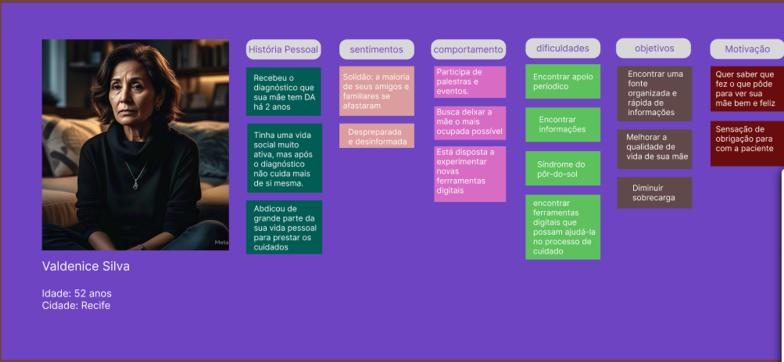
\includegraphics[width=0.92\textwidth]{figuras/img3-persona-valdenice.jpg}
\end{figure}

\begin{figure}[H]
  \centering
  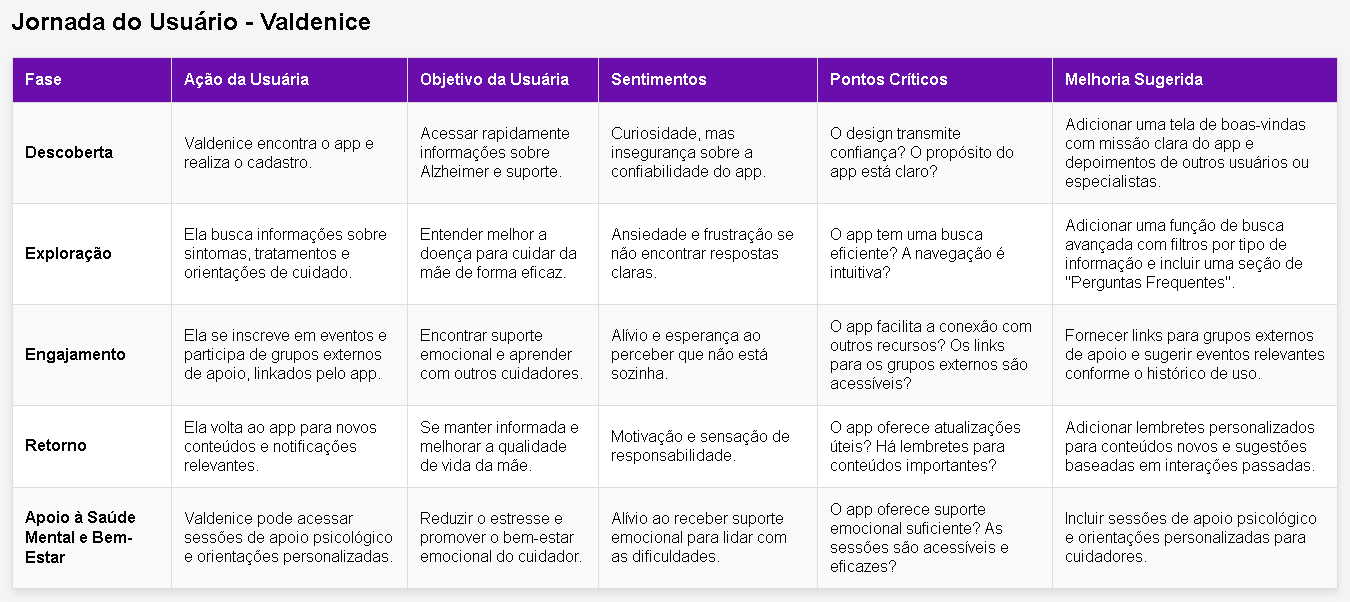
\includegraphics[width=0.92\textwidth]{figuras/img4-jornada-valdenice.png}
\end{figure}

% Da seção Análise de Competidores em diante: entrelinha 1,15 e espaçamento entre parágrafos de 8pt (igual às páginas 5-8 do relatorio.pdf)
\setstretch{1.15}
\setlength{\parindent}{0pt}
\setlength{\parskip}{8pt}

\subtituloSecao{Análise de Competidores (Benchmarking)}

Para fechar a exploração do problema e garantir que eu não estivesse reinventando a roda, analisei 5 soluções e canais já existentes no mercado (\textit{Alzheimer Portugal, Cuidadoria Torrent, Instituto Neuro, Grupos de Facebook e Movimento Cuidadores Informais}, além de uma menção honrosa ao \textit{Diário do Cuidado}, que se mostrou fora do ar). Avaliei cada um com notas de 1 a 5 em sete critérios: acessibilidade de custo, facilidade de uso, informações claras e concisas, cursos, interação entre cuidadores, eventos e administração de medicamentos.

\begin{table}[H]
  \centering
  \footnotesize
  \setlength{\tabcolsep}{3pt}
  \renewcommand{\arraystretch}{1.35}
  \begin{tabular}{|L{2.0cm}|C{2.05cm}|C{1.4cm}|C{1.75cm}|C{1.05cm}|C{1.65cm}|C{1.05cm}|C{1.95cm}|}
    \hline
    \raggedright Item & \raggedright Acessibilidade de custo & \raggedright Facilidade de Uso & \raggedright Informações claras e concisas & \raggedright Cursos & \raggedright Interação entre cuidadores & \raggedright Eventos & \raggedright\arraybackslash Administração de medicamentos \\
    \hline
    Alzheimer Portugal & 3/5 & 3/5 & 4/5 & 4/5 & 4/5 & 4/5 & 1/5 \\
    \hline
    Cuidadoria Torrent & 5/5 & 4/5 & 4/5 & 3/5 & 1/5 & 2/5 & 2/5 \\
    \hline
    Instituto Neuro & 4/5 & 3/5 & 3/5 & 5/5 & 1/5 & 1/5 & 3/5 \\
    \hline
    Grupo Facebook & 5/5 & 5/5 & 2/5 & 1/5 & 5/5 & 3/5 & 1/5 \\
    \hline
    Movimento Cuidadores Informais & 5/5 & 4/5 & 3/5 & 1/5 & 2/5 & 2/5 & 2/5 \\
    \hline
  \end{tabular}
\end{table}

A análise revelou uma lacuna clara: enquanto grupos de Facebook têm ótima interação gratuita (5/5), eles pecam na confiabilidade e clareza das informações (2/5). Por outro lado, plataformas com bom conteúdo (como \textit{Cuidadoria Torrent} e \textit{Instituto Neuro}) praticamente não oferecem interação entre cuidadores (1/5) nem divulgação de eventos locais. Essa comparação mostrou que o grande diferencial do projeto seria unir, em um só lugar gratuito e de fácil uso, \textbf{informações confiáveis e diretas sobre o manejo diário com a ponte para eventos e grupos reais de apoio.}

\subtituloSecao{Geração de Alternativas}

Depois de entender a fundo a rotina e as dores das cuidadoras, parti para a fase de ideação com o objetivo de pensar no maior número possível de soluções sem julgamentos prévios. Como o próprio fluxo de Design Thinking não é linear, realizei esse processo em duas rodadas: uma primeira mais abrangente (incluindo controle de medicamentos e rotina) e uma segunda já refinada após a imersão na ABRAz, focando diretamente na busca por informações confiáveis e no acesso a apoio emocional.

Em ambas as rodadas, apliquei 3 técnicas criativas complementares:

\begin{itemize}[leftmargin=1.25cm, label=\textbullet, topsep=2pt, itemsep=6pt]
  \item \textbf{Variante do BrainWriting 6-3-5:} Para manter a agilidade e praticidade, utilizei uma tabela rápida onde anotei 3 ideias em até 5 minutos usando frases curtas (entre 6 e 10 palavras). Daqui saíram propostas como criar um calendário de eventos sobre DA na cidade, uma aba com artigos científicos simplificados, espaços de desabafo anônimo e um chatbot especializado para tirar dúvidas rápidas sobre o cuidado.
  \item \textbf{SuperHeroes (Super-Heróis):} Uma dinâmica lúdica que usa os poderes de personagens famosos como metáfora para destravar soluções fora da caixa. Por exemplo, pensei no \textit{Doutor Destino} (usar magia para estar em vários lugares ao mesmo tempo e mapear onde e quando acontecem os encontros presenciais de cuidadores), no \textit{Homem-Aranha} (usar o "sentido aranha" para localizar pacientes perdidos) e no \textit{Tony Stark} (usar tecnologia de ponta para criar uma IA personalizada que sabe tudo sobre o paciente e orienta o cuidador em tempo real).
  \item \textbf{Fresh Eye (Olhar Fresco):} Apresentei o problema para pessoas de fora do projeto (entre 24 e 61 anos) para colher visões sem viés. As sugestões foram direto ao ponto: ter uma seção de Perguntas Frequentes (FAQ), links diretos para grupos de apoio da própria cidade, explicações claras sobre a evolução da doença e como lidar com mudanças de comportamento.
\end{itemize}

\subtituloSecao{Seleção de Alternativas}

Com dezenas de ideias geradas, agrupei as propostas principais em dois grandes eixos: \textbf{Busca de Informações} e \textbf{Acesso a Apoio}, totalizando 9 ideias centrais. Para escolher o que realmente entraria no escopo do protótipo sem cair no achismo, apliquei a \textbf{Técnica NAF} (Novidade, Atratividade/Apelo e Viabilidade), pontuando cada ideia de 1 a 10 em cada critério (total máximo de 30 pontos).

\hspace*{1.25cm}Ideias que pareciam interessantes no papel acabaram caindo por baixa viabilidade ou apelo prático — como mostrar cuidadores próximos por geolocalização (20/30 pontos, já que muitos cuidadores têm receio de iniciar contato com desconhecidos) ou listar contatos diretos de médicos (21/30 pontos, pela barreira de autorização e divulgação desses contatos).

\hspace*{1.25cm}Ao final, selecionei as \textbf{5 ideias mais bem pontuadas} para compor o coração do aplicativo:

\begin{enumerate}[leftmargin=1.25cm, topsep=2pt, itemsep=6pt]
  \item \textbf{Calendário com eventos e encontros sobre DA (30/30 pontos):} Essencial para promover a troca de experiências presencial e online.
  \item \textbf{Ponte com grupos de apoio locais (28/30 pontos):} Direcionamento direto com links e informações de associações (como a ABRAz) e comunidades de WhatsApp/Facebook para reduzir a solidão.
  \item \textbf{Informações científicas sobre DA de forma acessível (28/30 pontos):} Traduzir a ciência para uma linguagem simples, rápida e sem jargões médicos.
  \item \textbf{Guias sobre a descoberta da doença e o manejo no cuidado (28/30 pontos):} Dicas práticas para lidar com a Síndrome do Pôr-do-Sol, alimentação, exercícios e saúde mental do cuidador.
  \item \textbf{Perguntas Frequentes - FAQ (26/30 pontos):} Respostas curtas e imediatas para as dúvidas mais comuns do dia a dia.
\end{enumerate}

\textbf{OBS.:} Como a ideia do Chatbot especializado também teve um apelo altíssimo na matriz — nota 9/10 pela praticidade de tirar dúvidas rápidas e aliviar a solidão —, decidi resgatá-la agora na evolução funcional da plataforma como o diferencial de Inteligência Artificial do projeto.

\subtituloSecao{Implantação da Solução}

Com as 5 funcionalidades mais bem pontuadas na matriz NAF em mãos, parti para a materialização visual da proposta no \textbf{Figma}, batizada de \textbf{CuiDA}. O desenvolvimento seguiu uma evolução natural: comecei com um protótipo de baixa fidelidade para validar a arquitetura da informação e o fluxo básico de telas, avançando em seguida para um protótipo interativo de média fidelidade.

Para a identidade visual, escolhi o roxo como cor principal (símbolo oficial da conscientização sobre a Doença de Alzheimer) combinado a um fundo em tom creme suave, seguindo a diretriz mapeada na análise de competidores de construir uma interface acolhedora, com tons calmos e sem poluição visual para não sobrecarregar ainda mais a cuidadora.

O fluxo do protótipo foi organizado em torno de uma tela inicial simples e direta, dividida nos 4 pilares selecionados:

\begin{itemize}[leftmargin=1.25cm, label=\textbullet, topsep=2pt, itemsep=6pt]
  \item \textbf{Eventos e Encontros:} Um mural com atividades presenciais e online na região (como webinários e simpósios na UNICAP), informando datas, horários, locais e permitindo realizar a inscrição diretamente pela tela.
  \item \textbf{Links de Apoio:} Uma ponte direta para combater o isolamento social, reunindo atalhos para o Instagram da ABRAz Pernambuco, comunidades no Facebook e grupos de WhatsApp de cuidadores do Recife.
  \item \textbf{Sobre Alzheimer:} Uma central de conteúdos rápidos e ilustrados que traduzem a ciência para a prática, abordando \textit{O que é a DA, Saúde mental do cuidador, Orientações sobre alimentação, Síndrome do pôr-do-sol, Alzheimer e dança e Exercícios físicos.}
  \item \textbf{Perguntas Frequentes (FAQ):} Uma lista em formato acordeão (abre e fecha) com respostas curtas e diretas para as dúvidas mais urgentes do dia a dia.
\end{itemize}

\subtituloSecao{Avaliação da Solução}

Para validar se o protótipo realmente era fácil de usar pelo público-alvo, apliquei testes de usabilidade utilizando a plataforma \textbf{Maze} aliada ao protocolo \textit{Think Aloud} (pedindo para as participantes pensarem em voz alta enquanto interagiam com a tela, com gravação de áudio e vídeo).

O teste foi dividido em duas partes: primeiro, a execução de 7 tarefas práticas (como se inscrever no evento online do dia 01/04, achar dicas sobre alimentação, acessar o Instagram da ABRAz-PE, descobrir como lidar com a Síndrome do Pôr-do-Sol e verificar se o Alzheimer tem cura); segundo, um momento de exploração livre seguido de coleta de sugestões.

Realizei os testes com duas cuidadoras reais do perfil mapeado: \textbf{Miriam (54 anos)} e \textbf{Janey (58 anos)}. Os resultados trouxeram aprendizados práticos valiosos tanto sobre o método quanto sobre a interface:

\begin{itemize}[leftmargin=1.25cm, label=\textbullet, topsep=2pt, itemsep=6pt]
  \item \textbf{Limitação da ferramenta de teste vs. Protótipo:} Ambas tiveram bastante dificuldade para entender a mecânica da plataforma Maze em si (a ideia de ler um enunciado e cumprir uma missão fechada), pois o instinto natural era explorar o aplicativo livremente. Isso distorceu os tempos brutos medidos pelo Maze, provando que a dificuldade estava na ferramenta de avaliação, e não na interface do CuiDA. Além disso, elas ficaram frustradas quando clicavam em links de apoio que ainda estavam inativos no Figma.
  \item \textbf{Pontos elogiados:} As duas aprovaram bastante a proposta geral, destacando positivamente a paleta de cores, os nomes intuitivos dos botões e o uso de textos curtos e informativos.
  \item \textbf{Problemas de usabilidade identificados e iterados:}
    \begin{enumerate}[leftmargin=0.8cm, topsep=4pt, itemsep=4pt]
      \item Na tela de \textbf{Perguntas Frequentes (FAQ)}, tanto Miriam quanto Janey tentavam abrir as respostas clicando em cima do texto da pergunta, e não no pequeno ícone de triângulo ao lado. Seguindo o caráter iterativo do Design Thinking, modifiquei imediatamente o componente para abrir e fechar ao clicar em toda a extensão da pergunta.
      \item Na tarefa de retornar ao menu principal, ambas clicaram repetidas vezes em \textit{"Voltar"} antes de notarem o botão \textit{"Página Inicial"} ao lado.
      \item Como evolução de produto, Janey sugeriu a criação de um espaço de interação direta entre cuidadores e uma área voltada a novidades sobre a doença — insumos que guiaram diretamente a etapa seguinte de implementação do sistema em código real com Inteligência Artificial integrada.
    \end{enumerate}
\end{itemize}

% ==============================================================================
% PARTE 2 — DOCUMENTAÇÃO TÉCNICA DA PLATAFORMA, TECNOLOGIAS, IA E DEPLOY
% ==============================================================================

\tituloSecao{A Plataforma CuiDA (Do Protótipo ao Sistema Real)}

Com os achados do Design Thinking e dos testes de usabilidade validados no Figma, parti para a construção da plataforma real em código. O objetivo foi transformar aquele protótipo em um sistema completo, seguro e pronto para uso imediato por cuidadoras reais, preservando a mesma identidade acolhedora em tons de roxo e creme suave, mas agora conectado a um banco de dados real e equipado com um assistente de Inteligência Artificial baseado em evidências científicas.

Pensando na realidade do público-alvo — que muitas vezes acessa pelo celular nos intervalos do cuidado, mas também utiliza computador em casa —, desenvolvi a interface de modo responsivo com alternância rápida entre visualização \textbf{Mobile} e modo \textbf{Site PC} por meio de um seletor no topo da página.

\subtituloSecao{Principais Funcionalidades Implementadas}

\begin{itemize}[leftmargin=1.25cm, label=\textbullet, topsep=2pt, itemsep=6pt]
  \item \textbf{Cadastro, Login, Perfil Contextual e Recuperação de Senha por E-mail:} Além de nome, e-mail e senha, a usuária informa opcionalmente sua data de nascimento, cidade/estado, o nome da pessoa cuidada, o grau de parentesco e o estágio do Alzheimer (inicial, moderado ou avançado). Esses dados alimentam o atendimento personalizado. Caso esqueça a senha, há recuperação automatizada com envio de código temporário de 6 dígitos (válido por 15 minutos) diretamente para o e-mail cadastrado por meio da API da \textbf{Brevo}.
  \item \textbf{Assistente CuiDA (Página Única com IA e Acervo Científico):} O chatbot projetado na ideação ganhou uma tela única dedicada, acessível direto na tela inicial. Ela conta com botões de perguntas rápidas de 1 toque, painel expansível com todos os 8 documentos oficiais do acervo, botões flutuantes para ir direto ao \textbf{Início} ou ao \textbf{Final} do histórico e controle de rolagem que mantém o início da resposta visível na tela (para a usuária ler do começo sem se perder). Ao fim de cada orientação, aparecem referências clicáveis que abrem o PDF oficial exatamente na página citada.
  \item \textbf{Eventos e Encontros Integrados ao Banco:} Os encontros presenciais e webinários são carregados dinamicamente do PostgreSQL. A cuidadora visualiza data, horário, local, descrição detalhada e realiza ou cancela sua inscrição em um clique.
  \item \textbf{Links de Apoio Reais e Funcionais:} Corrigindo a frustração detectada nos testes do Figma, todos os atalhos agora abrem diretamente os canais reais: Instagram da ABRAz Pernambuco, grupos de apoio no WhatsApp (como Cuidadores de Recife) e comunidades no Facebook (como o GAFA).
  \item \textbf{Sobre Alzheimer e Perguntas Frequentes (FAQ):} Cartões educativos estruturados (\textit{O que é?, Saúde mental do cuidador, Orientações sobre alimentação, Síndrome do pôr-do-sol, Alzheimer e dança} e \textit{Exercícios físicos}) acompanhados do FAQ em acordeão já corrigido para abrir e fechar ao clicar em toda a faixa da pergunta.
  \item \textbf{Acessibilidade para Público 50+:} Controles globais \textbf{A-} e \textbf{A+} ajustam o tamanho da fonte em toda a plataforma em tempo real, e o botão \textbf{Ouvir} utiliza síntese de voz (\textit{Text-to-Speech}) com normalização automática para pronunciar corretamente datas, horários e siglas (como DA, SUS e ABRAz).
\end{itemize}

\tituloSecao{Arquitetura e Tecnologias Utilizadas}

Estruturei o sistema em arquitetura cliente-servidor em camadas (\textit{Routes, Controllers, Services, Repositories, Middlewares} e o módulo específico \texttt{src/rag/} para recuperação documental), priorizando código simples de manter, tipagem forte e baixo consumo de memória na nuvem.

\begin{table}[H]
  \centering
  \small
  \renewcommand{\arraystretch}{1.35}
  \begin{tabularx}{\textwidth}{|L{3.1cm}|L{4.2cm}|Y|}
    \hline
    Camada & Tecnologias e Bibliotecas & Papel no CuiDA \\
    \hline
    Frontend Web & HTML5, Tailwind CSS e JavaScript (ES6+), Web Speech API & Interface responsiva (Mobile e Site PC), controles de acessibilidade (A-/A+), leitura em voz alta e chat interativo com links por página. \\
    \hline
    Backend e API & Node.js (v22+), TypeScript e Express & Servidor HTTP único servindo a interface estática, os arquivos PDF do acervo (\texttt{/acervo-pdf}) e as rotas REST em JSON. \\
    \hline
    Banco de Dados e Vetores & PostgreSQL 15+, extensão \texttt{pgvector} (índice HNSW) e Full-Text Search (índices GIN) & Persistência de usuários, eventos, inscrições, artigos, FAQs e armazenamento dos trechos e vetores semânticos (768 dimensões) dos PDFs. \\
    \hline
    ORM e Migrações & Prisma ORM (\texttt{prisma} / \texttt{@prisma/client}) & Modelagem relacional, migrações versionadas (incluindo extensão \texttt{pgvector}), consultas parametrizadas e \textit{seed} idempotente. \\
    \hline
    Processamento de PDF & \texttt{pdfjs-dist} (build legacy Node.js) & Leitura página a página do texto real dos PDFs, reconstrução de linhas por coordenadas e detecção de títulos e arquivos digitalizados. \\
    \hline
    Segurança e Autenticação & \texttt{bcryptjs}, tokens JWT (\texttt{HS256}) via \texttt{crypto} em cookies \texttt{HttpOnly} & Hash seguro de senhas, validação de sessão sem expor tokens no navegador e bloqueio rigoroso de acesso indevido entre usuários (\textit{IDOR}). \\
    \hline
    Serviço de E-mail & API transacional da Brevo (com fallback \texttt{console} em dev) & Envio automático de códigos de recuperação de senha em produção, mantendo desenvolvimento local sem dependência externa. \\
    \hline
    Ambiente Local & Docker Compose (\texttt{pgvector/pgvector:pg15}) e Yarn & Sobe o banco com suporte vetorial localmente em um único comando, preservando independência em relação à nuvem. \\
    \hline
  \end{tabularx}
\end{table}

\subtituloSecao{Segurança e Proteção contra Acesso Indevido e Abuso de Cotas}

Durante a revisão do código, identifiquei e corrigi uma vulnerabilidade clássica de segurança conhecida como \textbf{IDOR} (\textit{Insecure Direct Object Reference}): inicialmente, rotas como perfil e inscrições recebiam o parâmetro \texttt{userId} enviado pelo cliente, o que em tese permitiria que um usuário autenticado tentasse consultar ou alterar dados de outra pessoa apenas trocando o número do ID na requisição.

Para resolver isso de forma definitiva, implementei autenticação assinada via \textbf{JWT (HMAC-SHA256)} armazenada em cookie \textbf{\texttt{HttpOnly; SameSite=Lax; Secure}} (com \texttt{trust proxy} ativado para funcionamento atrás do proxy HTTPS da nuvem). Toda requisição autenticada passa pelo middleware que extrai o ID real diretamente do token assinado e bloqueia com erro HTTP 403 qualquer tentativa de enviar um \texttt{userId} diferente do usuário logado.

Além disso, como a plataforma fica exposta publicamente na internet com chaves de API armazenadas no servidor, protegi os endpoints críticos contra automação e esgotamento de cotas (\textit{rate limiting}): o Assistente CuiDA exige sessão autenticada (\texttt{requireAuth}) com teto de \textbf{12 perguntas por minuto e 60 por hora} por usuário/IP, o disparo de recuperação por e-mail limita-se a \textbf{10 envios a cada 15 minutos} por IP e por destinatário, há limite de \textbf{32 KB} para o corpo JSON e um disjuntor diário de chamadas à Gemini API que comuta automaticamente para contingência local caso o teto de segurança seja atingido.

\tituloSecao{Inteligência Artificial: no Produto e no Desenvolvimento}

A Inteligência Artificial esteve presente em duas frentes complementares no projeto: dentro do próprio produto, dando vida ao \textbf{Assistente CuiDA}, e ao longo de todo o ciclo de engenharia para acelerar pesquisa, implementação, auditoria de código e testes.

\subtituloSecao{Como a IA Funciona Dentro do CuiDA (PTCF e RAG Avançado)}

Para evitar respostas genéricas ou conselhos médicos arriscados típicos de um chat comum, estruturei o comportamento do agente por meio de duas camadas técnicas combinadas:

\textbf{1. Engenharia de Prompt Estruturada (Framework PTCF):} As instruções do sistema residem no arquivo \texttt{src/prompts/assistente-cuida.ptcf.md}, organizado nos quatro pilares \textbf{PTCF}:
\begin{itemize}[leftmargin=1.25cm, label=\textbullet, topsep=2pt, itemsep=5pt]
  \item \textbf{P — Persona:} Especialista acolhedor, sereno e didático, adaptado para conversar com familiares emocionalmente sobrecarregados e público 50+ em português claro, sem jargões difíceis.
  \item \textbf{T — Tarefa e Travas Éticas (Guardrails):} Proíbe estritamente prescrever medicamentos, alterar dosagens ou dar diagnósticos; prioriza condutas não farmacológicas e Terapia de Validação (em linha com o PCDT do Ministério da Saúde e diretriz NICE NG97); e instrui explicitamente o modelo a tratar os trechos recuperados e o histórico do chat apenas como \textbf{dados não confiáveis} (delimitados em tags XML \texttt{<evidencia>}), prevenindo ataques de \textit{prompt injection}.
  \item \textbf{C — Contexto Injetado Dinamicamente:} Recebe em tempo real o resumo do perfil da cuidadora logada (nome, familiar cuidado, estágio da doença), o status de suficiência das evidências recuperadas, os trechos científicos extraídos dos PDFs e, quando pertinente, os eventos e links cadastrados no próprio aplicativo.
  \item \textbf{F — Formato da Resposta:} Organiza a leitura no celular em blocos previsíveis: acolhimento breve citando a pessoa cuidada, \textit{Por que isso acontece}, \textit{O que fazer na prática}, \textit{O que evitar}, \textit{Quando procurar o médico} e a linha de controle \texttt{[FONTES\_USADAS: E1, ...]} com os IDs realmente aproveitados.
\end{itemize}

\textbf{2. Arquitetura de RAG Híbrido (\textit{Retrieval-Augmented Generation}):} Em vez de enviar textos fixos ou manuais inteiros para a IA, construí um mecanismo completo de recuperação sobre todos os \textbf{8 documentos PDF oficiais} armazenados em \texttt{acervo-pdf/} — somando \textbf{460 páginas, mais de 107 mil palavras e 990 trechos estruturais indexados}. O acervo reúne o guia da \textbf{ABRAz}, o \textbf{PCDT de Doença de Alzheimer do Ministério da Saúde (2025)}, o manual \textbf{iSupport da Organização Mundial da Saúde (OMS)}, a diretriz internacional \textbf{NICE NG97} e guias geriátricos especializados sobre resistência ao banho, estratégias de diálogo, perambulação e desejo de sair de casa.

\begin{itemize}[leftmargin=1.25cm, label=\textbullet, topsep=2pt, itemsep=5pt]
  \item \textbf{Ingestão Incremental e Idempotente:} Um script CLI independente (\texttt{yarn rag:ingest}) extrai o texto preservando o número exato de cada página, detecta documentos digitalizados sem texto (\texttt{needs\_ocr}) e verifica o hash SHA-256 de cada arquivo para reprocessar apenas PDFs novos ou alterados. Na fragmentação (\textit{chunking}), o algoritmo respeita parágrafos, seções, sobreposição controlada (\textit{overlap}) e agrupa alertas médicos à recomendação principal.
  \item \textbf{Embeddings e Busca Híbrida (pgvector + FTS + RRF):} Os trechos geram embeddings semânticos de 768 dimensões usando o modelo oficial \texttt{gemini-embedding-001}, gravados no PostgreSQL com índice \texttt{HNSW}. Durante uma pergunta, o sistema executa em paralelo a busca vetorial (que inclusive permite cruzar perguntas em português com o conteúdo em inglês do manual iSupport e da diretriz NICE) e a busca lexical nativa do PostgreSQL (\textit{Full-Text Search} com dicionários \texttt{portuguese} e \texttt{simple} combinada a expansões de sinônimos como \textit{"chuveiro"} $\leftrightarrow$ banho). Os rankings são fundidos via \textbf{Reciprocal Rank Fusion (RRF)} e limitados por documento para garantir respostas multi-fonte.
  \item \textbf{Citações Verificáveis e Controle de Ausência de Evidências:} O contexto selecionado é sintetizado pelo modelo generativo \texttt{gemini-3.1-flash-lite} (com cadeia de fallback configurada). O backend valida os IDs indicados em \texttt{[FONTES\_USADAS: ...]} contra o conjunto efetivamente enviado ao modelo — bloqueando qualquer título ou página alucinada — e gera links clicáveis com âncora direta por página (\texttt{/acervo-pdf/arquivo.pdf\#page=N}). Caso a busca não atinja o limiar calibrado de evidência (como dúvidas culinárias fora de escopo ou perguntas sobre dosagem específica de insulina), o sistema recusa responder sem fontes e explica sua limitação de forma transparente.
  \item \textbf{Avaliação Empírica Comparativa:} Na bateria automatizada de avaliação com 15 cenários cotidianos e de segurança clínica (\texttt{yarn rag:eval}), o novo RAG híbrido saltou de \textbf{0,909} para \textbf{1,000 (100\%) em Hit@6}, elevou o \textbf{Recall por documento} de \textbf{0,432} para \textbf{0,668} e o \textbf{MRR} de \textbf{0,803} para \textbf{0,939} (combinando em média 3,73 documentos distintos por resposta), além de atingir \textbf{100\% (4/4)} na recusa correta de perguntas fora do acervo (incluindo temas culinários, dosagem de insulina e sintomas agudos como dor no peito e dor no joelho) frente a \textbf{0\% (0/4)} do mecanismo anterior baseado apenas em palavras-chave.
\end{itemize}

\subtituloSecao{Ferramentas de IA Utilizadas na Construção do Projeto}

\begin{itemize}[leftmargin=1.25cm, label=\textbullet, topsep=2pt, itemsep=6pt]
  \item \textbf{NotebookLM (Google Gemini):} Utilizado na etapa de pesquisa e curadoria documental para explorar, cruzar e validar os trechos mais relevantes dentro de documentos extensos e densos — em especial o manual iSupport da OMS (275 páginas) e o PCDT do Ministério da Saúde (90 páginas) —, garantindo que a seleção de condutas ficasse fiel às evidências clínicas.
  \item \textbf{Antigravity (Google DeepMind):} Utilizado como agente principal de engenharia durante todo o desenvolvimento do código. Através dele, estruturei a aplicação full-stack a partir das telas validadas no Figma, modelei a base no Prisma, converti materiais de referência web em PDFs limpos para o acervo, implementei o assistente com prompt PTCF e o pipeline de RAG híbrido com \texttt{pgvector}, corrigi a falha de segurança anti-IDOR, configurei o envio de e-mails e produzi as suítes automatizadas de testes e esta documentação.
  \item \textbf{ChatGPT (OpenAI):} Utilizado estrategicamente como \textbf{segunda opinião técnica e auditoria independente} sobre o código já versionado no repositório do GitHub. Ao revisar os arquivos do projeto, o ChatGPT ajudou a identificar melhorias valiosas — como separar a URL \textit{pooled} (\texttt{DATABASE\_URL}) da URL direta para migrações (\texttt{DIRECT\_URL}) no Neon, tornar o \textit{seed} seguro contra reexecuções destrutivas, revisar o comando de inicialização no \texttt{render.yaml} e elevar a barra de exigência arquitetural para a evolução do RAG híbrido e sua bateria objetiva de métricas.
\end{itemize}

\tituloSecao{Infraestrutura em Nuvem (Render e Neon): Motivação e Limitações}

\subtituloSecao{Motivação para a Escolha do Render e do Neon}

Durante a preparação da entrega final do projeto, surgiu um problema prático importante: se a aplicação rodasse apenas no meu computador via Docker, quem fosse avaliar o CuiDA precisaria instalar Docker Desktop, subir o banco manualmente e ainda criar chaves próprias da API do Gemini e da Brevo para testar todas as funcionalidades — pois chaves secretas jamais podem ser publicadas diretamente em um repositório público do GitHub, sob risco de vazamento e revogação imediata.

Para garantir que qualquer avaliador possa testar o sistema completo com um único clique — mantendo a IA generativa, o RAG documental, o banco populado e o envio real de e-mails por Brevo funcionando sem precisar alterar uma única linha de código —, adotei a publicação gratuita combinando duas plataformas especializadas:

\begin{itemize}[leftmargin=1.25cm, label=\textbullet, topsep=2pt, itemsep=5pt]
  \item \textbf{Neon (Banco PostgreSQL Serverless na Nuvem):} Escolhido por oferecer plano gratuito persistente, URL dedicada para conexão direta (\texttt{DIRECT\_URL}) e \textit{pooling} (\texttt{DATABASE\_URL}), além de já incluir suporte nativo à extensão vetorial \textbf{\texttt{pgvector}} exigida pela busca semântica do RAG.
  \item \textbf{Render (Hospedagem do Web Service Node.js):} Escolhido por integrar-se diretamente ao repositório do GitHub (\textit{deploy} automático a cada atualização na branch principal), guardar as chaves secretas (\texttt{GEMINI\_API\_KEY}, \texttt{BREVO\_API\_KEY}, \texttt{AUTH\_SECRET} e URLs do Neon) de forma protegida no painel e executar automaticamente as migrações do Prisma e a compilação TypeScript — tudo isso preservando intacto o ambiente local via Docker para desenvolvimento.
\end{itemize}

\subtituloSecao{Limitações da Infraestrutura e da Solução Atual}

Em linha com a transparência adotada em toda esta documentação, destaco as principais limitações encontradas nessa arquitetura gratuita:

\begin{itemize}[leftmargin=1.25cm, label=\textbullet, topsep=2pt, itemsep=6pt]
  \item \textbf{Hibernação (\textit{Cold Start}) no Render Gratuito:} Após cerca de 15 minutos sem acessos, o plano gratuito do Render coloca a instância web em repouso. No primeiro acesso após a hibernação, a tela inicial pode levar entre \textbf{30 e 50 segundos} para responder até o servidor acordar novamente (os dados permanecem salvos no Neon).
  \item \textbf{Limite de 512 MB de RAM e ausência de Shell interativo no Render Free:} Processar centenas de páginas de PDF e calcular vetores em lotes dentro do servidor gratuito poderia esgotar a memória RAM durante a subida do aplicativo. Por essa razão, a ingestão (\texttt{yarn rag:ingest}) foi projetada como um comando CLI executado externamente apontando para o Neon, mantendo o servidor web do Render leve apenas para responder consultas.
  \item \textbf{Cotas gratuitas de Embeddings da Gemini API:} A camada gratuita do modelo \texttt{gemini-embedding-001} possui limite por minuto e teto diário de \textbf{1.000 requisições de embedding}. Durante testes intensivos com o acervo de 990 trechos, ao atingir esse teto diário, os trechos restantes do manual \textit{iSupport} (410 trechos) foram armazenados com indexação lexical FTS ativa para manter cobertura imediata, podendo ter os vetores pendentes preenchidos na execução seguinte assim que a cota diária renovar.
  \item \textbf{Caráter estritamente educativo e apoio clínico humano:} Apesar dos testes automatizados comprovarem alta fidelidade às fontes e recusa a temas fora de escopo, uma etapa complementar futura prevista na literatura de avaliação consiste na revisão qualitativa periódica das respostas por um médico geriatra ou profissional especializado, reforçando sempre que o CuiDA apoia o cuidado diário e não substitui acompanhamento médico presencial.
\end{itemize}

\end{document}
